\documentclass[10pt,twocolumn]{article}

\usepackage{algorithm}
%\usepackage{moreverb}   
%\usepackage{longtable}
\usepackage{fancyhdr}
\usepackage{algorithmic}             
%\usepackage{algorithm}
%\usepackage{array}     
\usepackage{hyperref}
\usepackage{graphicx}
\usepackage{subfigure}
\usepackage{fullpage}
\usepackage{amsmath, amssymb, amsthm}
%\usepackage[framed,numbered,autolinebreaks,useliterate]{mcode}
%\usepackage{mathabx}
\usepackage{float}

\usepackage[margin=1in]{geometry}

\title{{\bf Intrusion Detection through Provenance-Based Histograms}}
\author{
    Kenny Yu\\
    Harvard University\\
    \href{mailto:kennyyu@college.harvard.edu}{\texttt{kennyyu@college.harvard.edu}}
  \and
    R. J. Aquino\\
    Harvard University\\
    \href{mailto:rjaquino@college.harvard.edu}{\texttt{rjaquino@college.harvard.edu}}
}
\date{CS261, Fall 2013}

\begin{document}

\maketitle

%%%%%%%%%%%%%%%%%%%%%%%%%%%%%%%%%%%%%%%%%%%%%%%%%%%%
% ABSTRACT
%

\begin{abstract}
TODO
\end{abstract}

%%%%%%%%%%%%%%%%%%%%%%%%%%%%%%%%%%%%%%%%%%%%%%%%%%%%
% INTRODUCTION
%

\section{Introduction}
Provenance is metadata that tracks the history of all changes to files. In provenance-aware storage systems like PASS \cite{pass} and PASSv2 \cite{passv2}, the file system automatically tracks all dependencies whenever a file is created, modified, or deleted. These dependencies include the command that was executed to modify the file, the environment of the command, and all input files. The generated provenance forms a directed acyclic graph of typed nodes (e.g. files, processes, pipes) with properties (e.g. name, execution time, pid) and typed edges (e.g. forked, input, versioning). 

To make sense of the large amounts of data, Macko et. al. have developed Orbiter, a tool to visualize provenance graphs with semantic zoom \cite{orbiter}. Margo et. al. have developed techniques to analyze large provenance graphs and to extract useful information from these graphs, including semantic file attributes \cite{fileattributes}. Using simple provenance statistics on nodes (e.g. neighbors, file count, process count, edge count) and features from \texttt{stat}, they determine with high accuracy the type of files (e.g. source files, configuration files). Furthermore, they have identified key properties of provenance graphs and developed new centrality metrics to perform local clustering of graphs, separating the huge provenance graphs into smaller semantic tasks or workloads \cite{clustering}.

Applications that require provenance collection typically place great emphasis on data integrity. Given this priority, a natural goal of provenance systems is to detect intrusions on the system. Somayaji et. al. have developed techniques for detecting intrusions based on system call sequences, and counteract these by exponentially delaying or aborting system calls, rendering the system useless for a malicious attacker \cite{somayaji}\cite{somayaji-recent}. These intrusions include exploiting vulnerabilities in the SSH daemon and sendmail to obtain a shell with root privileges. Somayaji's work relies on building a {\em normal} profile of a process, and then detecting when the process deviates from normal.

Given the extensive amount of data PASS collects on file-file, file-process, and process-process dependencies, it seems plausible to detect intrusions based on provenance data collected by PASS. Tariq et. al. generalize Somayaji's sequences of system calls to sequences of provenance system events \cite{correlated-anomalies} to develop an intrusion detection system (IDS) in a distributed system. Their system uses bloom filters to store hashes of $k$-tuples--representing a sequence of provenance events--and then use these bit vectors to correlate anomalies across multiple hosts. King et. al. have developed Backtrack \cite{backtrack}, a modified Linux kernel that tracks dependencies between operating system objects (files, processes, file names) in a similar fashion to PASS. Given an intrusion, Backtrack builds a backwards casual graph to determine the entry point of an intrusion, and they have extended Backtrack with forward causal graphs to determine possibly tainted files, processes, and hosts from an intrusion in a distributed system \cite{multihost}. However, their system does not find a way of detecting an intrusion. Lei et. al. build similar process-file dependency trees, which they call access trees, and define a compatibility function to compare access trees with the goal of predicting future file accesses based on the current access tree pattern \cite{fileprefetch}.

Despite the existing work to detect intrusions and anomalies, Cao et. al. argue that any intrusion detection system cannot always distinguish good behaviors from bad behaviors because users behave too randomly to have an accurate model of the user's behavior \cite{fuzzy}. They propose their fuzzy anomaly detection approach to extend the training models in existing intrusion detection systems to account for the inherent fuzzy nature of intrusion detection. When training an IDS, instead of assigning hard 0s or 1s for features, their approach provides a way to reliably map these features to weights in the interval $[0,1]$. 

In this paper, we present a technique to analyze existing provenance data to detect if an intrusion occurred. 

In particular, we generate statistical models of normal behavior, against which we can test a node of interest. These statiscal models are histograms of different graph statistics, and we use these histograms to generate kernel density estimations to evaluate a test node. The contributions of this paper are:
\begin{enumerate}
\item A histogram-based technique for using provenance data to detect intrustions
\item An analysis of the different intrusions that can be identified, and the types of provenance which best contribute to these detections
\item A cogent plan for future work for using provenance data to detect intrusions
\end{enumerate}

%%%%%%%%%%%%%%%%%%%%%%%%%%%%%%%%%%%%%%%%%%%%%%%%%%%%
% DESIGN
%

\section{Design and Implementation}
Here we present our intrusion detection technique: a general and extendable statistical method for analyzing and comparing provenance data. At a high level, we process a provenance data graph, generating a model of "normal" behavior for each process/file in the graph. Using this model, we can determine the likelihood that a given "test" node is normal or whether it deviates from normal behavior and is thus potentially an exploited or malicious program.
\subsection{Models}
Our approach requires statistical models to evaluate the normalcy of a test node. The statistical model we chose to use was a kernel density estimation (KDE), which estimates the probability density function of a value with unknown distribution. To create the KDE, we needed to provide counts of a particular statistic. In this way, for each statistic that we chose to collect, we would be able to evaluate a test node's normalcy according to that statistic. For example, we could then ask "Does node $X_n$ have a statistically believable number of output processes compared to the other $X$ nodes?"
\subsection{Provenance Statistics}
As described above, in order to generate a KDE model, we need some statistic to measure. As we expected intrusions to differ in terms of the statistics that would stand out, we needed to generate a large number of statistics, and a model for each. With regards to provenance nodes directly, we compiled the following statistics:
\begin{enumerate}
\item The number of input files to the node.
\item The number of input processes to the node.
\item The number of input pipes to the node.
\item The number of output files to the node.
\item The number of output processes to the node.
\item The number of ouput pipes to the node.
\item file\_in\_version ??? XXX
\item file\_out\_version ??? XXX
\end{enumerate}
For ease of computation and comparison, we treated the different node types (e.g. file, process, pipe) separately so that we actually had different counts for "input files to a file node" and "input files to a process node", for instance.
\subsection{Centrality Metrics}
In addition to the data that can be collected on the nodes directly, we could also compute clustering statistics by considering each node in the context of the larger graph. Using the methods espoused by Macko et al. \cite{clustering}, we could compute different centrality and clustering metrics for a node, which can then be tabulated into a histogram like the input/output counts above. 
KENNY TODO: EXPAND THIS
\subsection{Implementation}
The implementation of the above techniques consists of multiple Python files, spanning about 850 lines of (commented) code. The raw BerkeleyDB database generated by PASS is provided as input, and textual/graphical results are outputted.
KENNY TODO: EXPAND THIS



%%%%%%%%%%%%%%%%%%%%%%%%%%%%%%%%%%%%%%%%%%%%%%%%%%%%
% EVALUATION
%

\section{Evaluation}

\subsection{Evaluation Methodology}
In order to test our techniques, we needed to run “exploits” on our PASS-enabled machine. We looked to prior work to get a sense of the different types of techniques commonly used to exploit security vulnerabilities. Commonly, remote network techniques [CITE DUKE PAPER] are used to broach insecure systems. Metasploit [CITE] is a software package designed to facilitate running exploits on insecure system. Searching the Metasploit database, as well as the online Exploit Database (exploit-db.com) [CITE], we found that most successful techniques involve exploiting vulnerabilities in software that a target system is running, as opposed to vulnerabilities in the target system itself. Put another way, we sought to exploit software packages, like mcrypt and gcc, not the Linux kernel itself. 

We found that many of the popular exploits involved buffer overflows and arbitrary code execution. Programming bugs in a piece of software allowed a malicious user, sending well-crafted data, to run arbitrary code on the target system. In particular, the mcrypt encryption package had a long standing buffer overflow, which would allow a malicious user to run their own code when mcrypt tried to decrypt the crafted exploit file. Due to limitations in our Virtual Machine set up, we were unable to exploit the vulnerable version of mcrypt, much like [CITE DUKE]. To emulate this exploit, we designed our own program, which would decrypt (via ROT13) an input file. When sent a particular “exploit file” which contained malicious lines, our program would stop decrypting and start running the code specified in the file.

Another type of exploit is more reminiscent of a system administration failure. If a malicious user replaces a program in /usr/bin, it could be used to log user actions. To emulate this sort of attack, we replaced /usr/bin/gcc with our own version of gcc, which, in addition to compiling the user’s code (via a call to gcc), logs that the user has made a request and copies the files the user had tried to compile. 

To generate the provenance data necessary to run the above analyses, we needed to run both “good” and “exploited” versions of our programs. For the mcrypt example, we ran our program on over 200 “good” inputs, and stored the provenance data. We then ran our program on two “bad” inputs, first to call “ls” as a Proof of Concept, and again to call “/bin/sh” to demonstrate that more severe attacks can be performed. We again exported the provenance generated by these steps, for comparison with our “good” usage. This is similar to recording all uses of a program during a server’s lifetime. 

For our system administration attack, we compiled the PASS toolset using GCC, and exported the provenance from these runs. We then replaced GCC with our exploited version, and compiled a few files, and exported the provenance again. In this way, we again acquired provenance for “normal” usage, before acquiring provenance for our attempted exploit. 


\subsection{Results}
\subsection{Provenance Data}
After running the normal and exploited programs described above, we visualized the provenance graphs using Orbiter \cite{orbiter}. After searching for the nodes named after our programs, we were able to find both the clean and exploited nodes. The clean nodes for "hello" simply read in one file through a pipe and outputted one file, whereas the exploited version clearly has a forked "/usr/bin/ls" process. Similarly, the mcrypt simulation (implemented in Python) has only an output file as a descendent normally, but when exploited has multiple extra processes/files as descendents (see Figure 1). Similarly, the normal GCC and exploited GCC displayed very different provenance graphs. 
\begin{figure*}
  \caption{Descendents of an unexploited mcrypt-style program. Simply an output file. Below, descendents of an exploited mcrypt-style program. In addition to an (offscreen) output file, there is also an outgoing /bin/sh process, with its own children.}
  \centering
    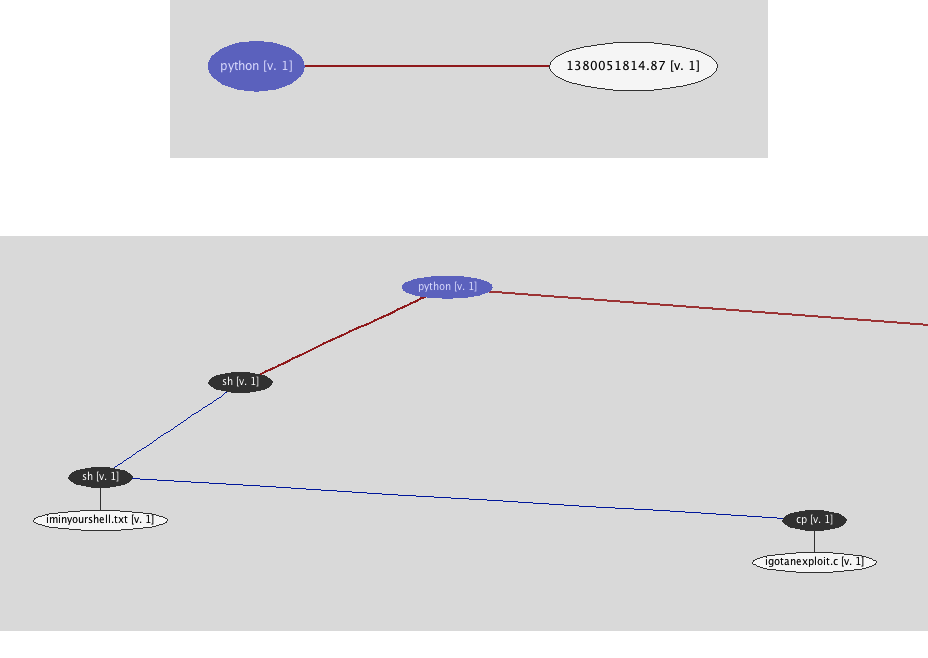
\includegraphics[width=\textwidth]{img/mcrypt.png}
\end{figure*}

\subsection{Statistical Data}
\subsection{KDE Predictions}
TODO:
true positives.
false positives.
graphs?

\subsection{Discussion}
TODO: 
why the numbers are the way they are.
what types of intrusions can we detect.
which provenance data is most useful

%%%%%%%%%%%%%%%%%%%%%%%%%%%%%%%%%%%%%%%%%%%%%%%%%%%%
% CONCLUSION
%

\section{Conclusion and Future Work}
TODO
not realtime. can it be made to detect intrusions in realtime?

%%%%%%%%%%%%%%%%%%%%%%%%%%%%%%%%%%%%%%%%%%%%%%%%%%%%
% BIBLIOGRAPHY
%

\begin{thebibliography}{99}

\bibitem{fuzzy}
\textsc{Cao, D., Qiu, M., Chen, Z., Hu, F., Zhu, Y., and Wang, B.} Intelligent Fuzzy Anomaly Detection of Malicious Software. In {\em Internal Journal of Advanced Intelligence}, vol. 4, no. 1, pp 69-86 (December 2012).

\bibitem{somayaji-recent}
\textsc{Inoue, H. and Somayaji, A.} Lookahead Pairs and Full Sequences: A Tale of Two Anomaly Detection Methods. In {\em 2nd Annual Symposium on Information Assurance} (June 2007). 

\bibitem{backtrack}
\textsc{King, S. T. and Chen, P. M.} Backtracking Intrusions. In {\em SOSP'03 Proceedings of the nineteenth ACM symposium on Operating systems principles} (December 2003).

\bibitem{multihost}
\textsc{King, S. T., Mao Z. M., Lucchetti, D. G., and Chen, P. M.} Enriching intrusion alerts through multi-host causality. In {\em Proceedings of the 2005 Network and Distributed System Security Symposium} (February 2005).

\bibitem{fileprefetch}
\textsc{Lei, H. and Duchamp, D.} An Analytical Approach to File Prefetching. In {\em Proceedings of the USENIX 1997 Annual Technical Conference} (January 1997).

\bibitem{clustering}
\textsc{Macko, P., Margo, D., Seltzer, M.} Local Clustering in Provenance Graphs (Extended Version). In {\em Proceedings of the 22nd ACM international conference on Conference on information \& knowledge management} (August 2013).

\bibitem{orbiter}
\textsc{Macko, P. and Seltzer, M.} Provenance Map Orbiter: Interactive Exploration of Large Provenance Graphs. In {\em TaPP'11 Proceedings of the 2nd conference on Theory and practice of provenance} (June 2011).

\bibitem{fileattributes}
\textsc{Margo, D., and Smogor, R.} Using Provenance to Extract Semantic File Attributes. In {\em TaPP'10 Proceedings of the 2nd conference on Theory and practice of provenance} (February 2010).

\bibitem{passv2}
\textsc{Muniswamy-Reddy, K., Braun, U., Holland, D. A., Macko, P., Maclean, D., Margo, D., Seltzer, M., and Smogor, R.} Layering in Provenance Systems. In {\em Proceedings of the 2009 USENIX Annual Technical Conference} (June 2009).

\bibitem{pass}
\textsc{Muniswamy-Reddy, K., Holland, D. A., Braun, U., and Seltzer, M.} Provenance-Aware Storage Systems. In {\em Proceedings of the 2006 USENIX Annual Technical Conference} (June 2006).

\bibitem{somayaji}
\textsc{Somayaji, A. and Forrest, S.} Automated Response Using System-Call Delays. In {\em Proceedings of the 2000 USENIX Annual Technical Conference} (August 2000).

\bibitem{correlated-anomalies}
\textsc{Tariq, D., Baig, B., Gehani, A., Mahmood, S., Tahir, R., Aqil, A., and Zaffar, F.} Identifying the provenance of correlated anomalies. In {\em SAC'11 Proceedings of the 2011 ACM Symposium on Applied Computing} (March 2011).

\end{thebibliography}

\end{document}
